\batchmode
\documentclass[a4paper]{book}
\usepackage{makeidx}
\usepackage{natbib}
\usepackage{graphicx}
\usepackage{multicol}
\usepackage{float}
\usepackage{listings}
\usepackage{color}
\usepackage{ifthen}
\usepackage[table]{xcolor}
\usepackage{textcomp}
\usepackage{alltt}
\usepackage[utf8]{inputenc}
\usepackage{mathptmx}
\usepackage[scaled=.90]{helvet}
\usepackage{courier}
\usepackage{sectsty}
\usepackage[titles]{tocloft}
\usepackage{doxygen}
\lstset{language=C++,inputencoding=utf8,basicstyle=\footnotesize,breaklines=true,breakatwhitespace=true,tabsize=8,numbers=left }
\makeindex
\setcounter{tocdepth}{3}
\renewcommand{\footrulewidth}{0.4pt}
\renewcommand{\familydefault}{\sfdefault}
\hfuzz=15pt
\setlength{\emergencystretch}{15pt}
\hbadness=750
\tolerance=750
\begin{document}
\begin{titlepage}
\vspace*{7cm}
\begin{center}
{\Large oryx\-\_\-srr\-\_\-gui }\\
\vspace*{1cm}
{\large \-Generated by Doxygen 1.7.6.1}\\
\vspace*{0.5cm}
{\small Sun Jan 27 2013 20:35:05}\\
\end{center}
\end{titlepage}
\clearemptydoublepage
\pagenumbering{roman}
\tableofcontents
\clearemptydoublepage
\pagenumbering{arabic}
\chapter{\-Main \-Page}
\label{index}

{\bfseries \doxyref{oryxsrr\-\_\-msgs}{p.}{namespaceoryxsrr__msgs}} 

-\/-\/$>$ 
\chapter{\-Namespace \-Index}
\section{\-Namespace \-List}
\-Here is a list of all namespaces with brief descriptions\-:\begin{DoxyCompactList}
\item\contentsline{section}{{\bf oryx\-\_\-srr\-\_\-gui} }{\pageref{namespaceoryx__srr__gui}}{}
\end{DoxyCompactList}

\chapter{\-Class \-Index}
\section{\-Class \-List}
\-Here are the classes, structs, unions and interfaces with brief descriptions\-:\begin{DoxyCompactList}
\item\contentsline{section}{{\bf oryx\-\_\-srr\-\_\-gui\-::\-Main\-Window} \\*\-Qt central, all operations relating to the view part here }{\pageref{classoryx__srr__gui_1_1MainWindow}}{}
\item\contentsline{section}{{\bf oryx\-\_\-srr\-\_\-gui\-::\-Q\-Node} }{\pageref{classoryx__srr__gui_1_1QNode}}{}
\end{DoxyCompactList}

\chapter{\-File \-Index}
\section{\-File \-List}
\-Here is a list of all files with brief descriptions\-:\begin{DoxyCompactList}
\item\contentsline{section}{{\bf occupancy\-\_\-generator.\-cpp} \\*\-Simple node for generating test occupancy grids }{\pageref{occupancy__generator_8cpp}}{}
\item\contentsline{section}{{\bf \-Occupancy\-Grid.\-cpp} \\*\-Contains the implementations for \doxyref{\-Occupancy\-Grid.\-h}{p.}{OccupancyGrid_8h} }{\pageref{OccupancyGrid_8cpp}}{}
\item\contentsline{section}{{\bf \-Occupancy\-Grid.\-h} \\*//\-T\-O\-D\-O fill in detailed discription here }{\pageref{OccupancyGrid_8h}}{}
\item\contentsline{section}{{\bf orxy\-\_\-path\-\_\-planning\-\_\-test.\-cpp} \\*\-Simple test node }{\pageref{orxy__path__planning__test_8cpp}}{}
\item\contentsline{section}{{\bf oryx\-\_\-global\-\_\-planner.\-cpp} \\*//\-T\-O\-D\-O fill in detailed discription here }{\pageref{oryx__global__planner_8cpp}}{}
\item\contentsline{section}{{\bf oryx\-\_\-local\-\_\-planner.\-cpp} }{\pageref{oryx__local__planner_8cpp}}{}
\item\contentsline{section}{{\bf \-Oryx\-Path\-Planning.\-h} \\*\-Contains all of the \-Includes required to complete the \doxyref{oryx\-\_\-path\-\_\-planning}{p.}{namespaceoryx__path__planning} namespace }{\pageref{OryxPathPlanning_8h}}{}
\item\contentsline{section}{{\bf \-Oryx\-Path\-Planning\-Utilities.\-h} \\*\-Header containing definitions that are used throughout the \doxyref{oryx\-\_\-path\-\_\-planning}{p.}{namespaceoryx__path__planning} package }{\pageref{OryxPathPlanningUtilities_8h}}{}
\item\contentsline{section}{{\bf \-Point\-Converter.\-hpp} \\*\-Header containg class definitions for converting between points }{\pageref{PointConverter_8hpp}}{}
\item\contentsline{section}{{\bf \-Tentacle\-\_\-test.\-cpp} }{\pageref{Tentacle__test_8cpp}}{}
\item\contentsline{section}{{\bf \-Tentacles.\-cpp} }{\pageref{Tentacles_8cpp}}{}
\item\contentsline{section}{{\bf \-Tentacles.\-h} }{\pageref{Tentacles_8h}}{}
\item\contentsline{section}{{\bf \-Type\-Definitions.\-h} \\*\-Common typedefs for the \doxyref{oryx\-\_\-path\-\_\-planning}{p.}{namespaceoryx__path__planning} namespace }{\pageref{TypeDefinitions_8h}}{}
\end{DoxyCompactList}

\chapter{\-Namespace \-Documentation}
\section{oryx\-\_\-srr\-\_\-gui \-Namespace \-Reference}
\label{namespaceoryx__srr__gui}\index{oryx\-\_\-srr\-\_\-gui@{oryx\-\_\-srr\-\_\-gui}}
\subsection*{\-Classes}
\begin{DoxyCompactItemize}
\item 
class {\bf \-Main\-Window}
\begin{DoxyCompactList}\small\item\em \-Qt central, all operations relating to the view part here. \end{DoxyCompactList}\item 
class {\bf \-Q\-Node}
\end{DoxyCompactItemize}

\chapter{\-Class \-Documentation}
\section{oryx\-\_\-srr\-\_\-gui\-:\-:\-Main\-Window \-Class \-Reference}
\label{classoryx__srr__gui_1_1MainWindow}\index{oryx\-\_\-srr\-\_\-gui\-::\-Main\-Window@{oryx\-\_\-srr\-\_\-gui\-::\-Main\-Window}}


\-Qt central, all operations relating to the view part here.  




{\ttfamily \#include $<$main\-\_\-window.\-hpp$>$}

\subsection*{\-Public \-Slots}
\begin{DoxyCompactItemize}
\item 
void {\bf on\-\_\-action\-About\-\_\-triggered} ()
\item 
void {\bf on\-\_\-button\-\_\-connect\-\_\-clicked} (bool check)
\item 
void {\bf on\-\_\-checkbox\-\_\-use\-\_\-environment\-\_\-state\-Changed} (int state)
\item 
void {\bf update\-Logging\-View} ()
\end{DoxyCompactItemize}
\subsection*{\-Public \-Member \-Functions}
\begin{DoxyCompactItemize}
\item 
void {\bf close\-Event} (\-Q\-Close\-Event $\ast$event)
\item 
{\bf \-Main\-Window} (int argc, char $\ast$$\ast$argv, \-Q\-Widget $\ast$parent=0)
\item 
void {\bf \-Read\-Settings} ()
\item 
void {\bf show\-No\-Master\-Message} ()
\item 
void {\bf \-Write\-Settings} ()
\item 
{\bf $\sim$\-Main\-Window} ()
\end{DoxyCompactItemize}
\subsection*{\-Private \-Attributes}
\begin{DoxyCompactItemize}
\item 
{\bf \-Q\-Node} {\bf qnode}
\item 
\-Ui\-::\-Main\-Window\-Design {\bf ui}
\end{DoxyCompactItemize}


\subsection{\-Detailed \-Description}
\-Qt central, all operations relating to the view part here. 

\-Definition at line 31 of file main\-\_\-window.\-hpp.



\subsection{\-Constructor \& \-Destructor \-Documentation}
\index{oryx\-\_\-srr\-\_\-gui\-::\-Main\-Window@{oryx\-\_\-srr\-\_\-gui\-::\-Main\-Window}!\-Main\-Window@{\-Main\-Window}}
\index{\-Main\-Window@{\-Main\-Window}!oryx_srr_gui::MainWindow@{oryx\-\_\-srr\-\_\-gui\-::\-Main\-Window}}
\subsubsection[{\-Main\-Window}]{\setlength{\rightskip}{0pt plus 5cm}{\bf oryx\-\_\-srr\-\_\-gui\-::\-Main\-Window\-::\-Main\-Window} (
\begin{DoxyParamCaption}
\item[{int}]{argc, }
\item[{char $\ast$$\ast$}]{argv, }
\item[{\-Q\-Widget $\ast$}]{parent = {\ttfamily 0}}
\end{DoxyParamCaption}
)}\label{classoryx__srr__gui_1_1MainWindow_a5dadb1deb81e4a78df82b71f44b365ab}


\-Definition at line 29 of file main\-\_\-window.\-cpp.

\index{oryx\-\_\-srr\-\_\-gui\-::\-Main\-Window@{oryx\-\_\-srr\-\_\-gui\-::\-Main\-Window}!$\sim$\-Main\-Window@{$\sim$\-Main\-Window}}
\index{$\sim$\-Main\-Window@{$\sim$\-Main\-Window}!oryx_srr_gui::MainWindow@{oryx\-\_\-srr\-\_\-gui\-::\-Main\-Window}}
\subsubsection[{$\sim$\-Main\-Window}]{\setlength{\rightskip}{0pt plus 5cm}{\bf oryx\-\_\-srr\-\_\-gui\-::\-Main\-Window\-::$\sim$\-Main\-Window} (
\begin{DoxyParamCaption}
{}
\end{DoxyParamCaption}
)}\label{classoryx__srr__gui_1_1MainWindow_a9bf3f79697decd32ab4e8d0a34a8d261}


\-Definition at line 55 of file main\-\_\-window.\-cpp.



\subsection{\-Member \-Function \-Documentation}
\index{oryx\-\_\-srr\-\_\-gui\-::\-Main\-Window@{oryx\-\_\-srr\-\_\-gui\-::\-Main\-Window}!close\-Event@{close\-Event}}
\index{close\-Event@{close\-Event}!oryx_srr_gui::MainWindow@{oryx\-\_\-srr\-\_\-gui\-::\-Main\-Window}}
\subsubsection[{close\-Event}]{\setlength{\rightskip}{0pt plus 5cm}void {\bf oryx\-\_\-srr\-\_\-gui\-::\-Main\-Window\-::close\-Event} (
\begin{DoxyParamCaption}
\item[{\-Q\-Close\-Event $\ast$}]{event}
\end{DoxyParamCaption}
)}\label{classoryx__srr__gui_1_1MainWindow_a5f3a1bc384611b61ef90e789c8fac987}


\-Definition at line 164 of file main\-\_\-window.\-cpp.

\index{oryx\-\_\-srr\-\_\-gui\-::\-Main\-Window@{oryx\-\_\-srr\-\_\-gui\-::\-Main\-Window}!on\-\_\-action\-About\-\_\-triggered@{on\-\_\-action\-About\-\_\-triggered}}
\index{on\-\_\-action\-About\-\_\-triggered@{on\-\_\-action\-About\-\_\-triggered}!oryx_srr_gui::MainWindow@{oryx\-\_\-srr\-\_\-gui\-::\-Main\-Window}}
\subsubsection[{on\-\_\-action\-About\-\_\-triggered}]{\setlength{\rightskip}{0pt plus 5cm}void {\bf oryx\-\_\-srr\-\_\-gui\-::\-Main\-Window\-::on\-\_\-action\-About\-\_\-triggered} (
\begin{DoxyParamCaption}
{}
\end{DoxyParamCaption}
)\hspace{0.3cm}{\ttfamily  [slot]}}\label{classoryx__srr__gui_1_1MainWindow_af41a67a96c68dddbae87dfd2edc588ce}


\-Definition at line 123 of file main\-\_\-window.\-cpp.

\index{oryx\-\_\-srr\-\_\-gui\-::\-Main\-Window@{oryx\-\_\-srr\-\_\-gui\-::\-Main\-Window}!on\-\_\-button\-\_\-connect\-\_\-clicked@{on\-\_\-button\-\_\-connect\-\_\-clicked}}
\index{on\-\_\-button\-\_\-connect\-\_\-clicked@{on\-\_\-button\-\_\-connect\-\_\-clicked}!oryx_srr_gui::MainWindow@{oryx\-\_\-srr\-\_\-gui\-::\-Main\-Window}}
\subsubsection[{on\-\_\-button\-\_\-connect\-\_\-clicked}]{\setlength{\rightskip}{0pt plus 5cm}void {\bf oryx\-\_\-srr\-\_\-gui\-::\-Main\-Window\-::on\-\_\-button\-\_\-connect\-\_\-clicked} (
\begin{DoxyParamCaption}
\item[{bool}]{check}
\end{DoxyParamCaption}
)\hspace{0.3cm}{\ttfamily  [slot]}}\label{classoryx__srr__gui_1_1MainWindow_a9912d7a78ec67447fc3ed485d89e94bc}


\-Definition at line 73 of file main\-\_\-window.\-cpp.

\index{oryx\-\_\-srr\-\_\-gui\-::\-Main\-Window@{oryx\-\_\-srr\-\_\-gui\-::\-Main\-Window}!on\-\_\-checkbox\-\_\-use\-\_\-environment\-\_\-state\-Changed@{on\-\_\-checkbox\-\_\-use\-\_\-environment\-\_\-state\-Changed}}
\index{on\-\_\-checkbox\-\_\-use\-\_\-environment\-\_\-state\-Changed@{on\-\_\-checkbox\-\_\-use\-\_\-environment\-\_\-state\-Changed}!oryx_srr_gui::MainWindow@{oryx\-\_\-srr\-\_\-gui\-::\-Main\-Window}}
\subsubsection[{on\-\_\-checkbox\-\_\-use\-\_\-environment\-\_\-state\-Changed}]{\setlength{\rightskip}{0pt plus 5cm}void {\bf oryx\-\_\-srr\-\_\-gui\-::\-Main\-Window\-::on\-\_\-checkbox\-\_\-use\-\_\-environment\-\_\-state\-Changed} (
\begin{DoxyParamCaption}
\item[{int}]{state}
\end{DoxyParamCaption}
)\hspace{0.3cm}{\ttfamily  [slot]}}\label{classoryx__srr__gui_1_1MainWindow_ae37883cff54b2286a87a5dbb22b16f6b}


\-Definition at line 94 of file main\-\_\-window.\-cpp.

\index{oryx\-\_\-srr\-\_\-gui\-::\-Main\-Window@{oryx\-\_\-srr\-\_\-gui\-::\-Main\-Window}!\-Read\-Settings@{\-Read\-Settings}}
\index{\-Read\-Settings@{\-Read\-Settings}!oryx_srr_gui::MainWindow@{oryx\-\_\-srr\-\_\-gui\-::\-Main\-Window}}
\subsubsection[{\-Read\-Settings}]{\setlength{\rightskip}{0pt plus 5cm}void {\bf oryx\-\_\-srr\-\_\-gui\-::\-Main\-Window\-::\-Read\-Settings} (
\begin{DoxyParamCaption}
{}
\end{DoxyParamCaption}
)}\label{classoryx__srr__gui_1_1MainWindow_a78e24c0c91671f5f9ecea34e536fe021}


\-Definition at line 131 of file main\-\_\-window.\-cpp.

\index{oryx\-\_\-srr\-\_\-gui\-::\-Main\-Window@{oryx\-\_\-srr\-\_\-gui\-::\-Main\-Window}!show\-No\-Master\-Message@{show\-No\-Master\-Message}}
\index{show\-No\-Master\-Message@{show\-No\-Master\-Message}!oryx_srr_gui::MainWindow@{oryx\-\_\-srr\-\_\-gui\-::\-Main\-Window}}
\subsubsection[{show\-No\-Master\-Message}]{\setlength{\rightskip}{0pt plus 5cm}void {\bf oryx\-\_\-srr\-\_\-gui\-::\-Main\-Window\-::show\-No\-Master\-Message} (
\begin{DoxyParamCaption}
{}
\end{DoxyParamCaption}
)}\label{classoryx__srr__gui_1_1MainWindow_a0e8e0a92c91b264d98e6bd33230a66ee}


\-Definition at line 61 of file main\-\_\-window.\-cpp.

\index{oryx\-\_\-srr\-\_\-gui\-::\-Main\-Window@{oryx\-\_\-srr\-\_\-gui\-::\-Main\-Window}!update\-Logging\-View@{update\-Logging\-View}}
\index{update\-Logging\-View@{update\-Logging\-View}!oryx_srr_gui::MainWindow@{oryx\-\_\-srr\-\_\-gui\-::\-Main\-Window}}
\subsubsection[{update\-Logging\-View}]{\setlength{\rightskip}{0pt plus 5cm}void {\bf oryx\-\_\-srr\-\_\-gui\-::\-Main\-Window\-::update\-Logging\-View} (
\begin{DoxyParamCaption}
{}
\end{DoxyParamCaption}
)\hspace{0.3cm}{\ttfamily  [slot]}}\label{classoryx__srr__gui_1_1MainWindow_a6d2c51c41173320def884b4e6d3d8e12}
\-This function is signalled by the underlying model. \-When the model changes, this will drop the cursor down to the last line in the \-Q\-Listview to ensure the user can always see the latest log message. 

\-Definition at line 115 of file main\-\_\-window.\-cpp.

\index{oryx\-\_\-srr\-\_\-gui\-::\-Main\-Window@{oryx\-\_\-srr\-\_\-gui\-::\-Main\-Window}!\-Write\-Settings@{\-Write\-Settings}}
\index{\-Write\-Settings@{\-Write\-Settings}!oryx_srr_gui::MainWindow@{oryx\-\_\-srr\-\_\-gui\-::\-Main\-Window}}
\subsubsection[{\-Write\-Settings}]{\setlength{\rightskip}{0pt plus 5cm}void {\bf oryx\-\_\-srr\-\_\-gui\-::\-Main\-Window\-::\-Write\-Settings} (
\begin{DoxyParamCaption}
{}
\end{DoxyParamCaption}
)}\label{classoryx__srr__gui_1_1MainWindow_a295afab25a5a11ee8cb260804f272c05}


\-Definition at line 152 of file main\-\_\-window.\-cpp.



\subsection{\-Member \-Data \-Documentation}
\index{oryx\-\_\-srr\-\_\-gui\-::\-Main\-Window@{oryx\-\_\-srr\-\_\-gui\-::\-Main\-Window}!qnode@{qnode}}
\index{qnode@{qnode}!oryx_srr_gui::MainWindow@{oryx\-\_\-srr\-\_\-gui\-::\-Main\-Window}}
\subsubsection[{qnode}]{\setlength{\rightskip}{0pt plus 5cm}{\bf \-Q\-Node} {\bf oryx\-\_\-srr\-\_\-gui\-::\-Main\-Window\-::qnode}\hspace{0.3cm}{\ttfamily  [private]}}\label{classoryx__srr__gui_1_1MainWindow_a9ec4eebaba280008a644bc994e3a2c2b}


\-Definition at line 59 of file main\-\_\-window.\-hpp.

\index{oryx\-\_\-srr\-\_\-gui\-::\-Main\-Window@{oryx\-\_\-srr\-\_\-gui\-::\-Main\-Window}!ui@{ui}}
\index{ui@{ui}!oryx_srr_gui::MainWindow@{oryx\-\_\-srr\-\_\-gui\-::\-Main\-Window}}
\subsubsection[{ui}]{\setlength{\rightskip}{0pt plus 5cm}\-Ui\-::\-Main\-Window\-Design {\bf oryx\-\_\-srr\-\_\-gui\-::\-Main\-Window\-::ui}\hspace{0.3cm}{\ttfamily  [private]}}\label{classoryx__srr__gui_1_1MainWindow_a1793f5a07bbfb5e354f48eb2fd08e5e9}


\-Definition at line 58 of file main\-\_\-window.\-hpp.



\-The documentation for this class was generated from the following files\-:\begin{DoxyCompactItemize}
\item 
{\bf main\-\_\-window.\-hpp}\item 
{\bf main\-\_\-window.\-cpp}\end{DoxyCompactItemize}

\section{oryx\-\_\-srr\-\_\-gui\-:\-:\-Q\-Node \-Class \-Reference}
\label{classoryx__srr__gui_1_1QNode}\index{oryx\-\_\-srr\-\_\-gui\-::\-Q\-Node@{oryx\-\_\-srr\-\_\-gui\-::\-Q\-Node}}


{\ttfamily \#include $<$qnode.\-hpp$>$}

\subsection*{\-Public \-Types}
\begin{DoxyCompactItemize}
\item 
enum {\bf \-Log\-Level} \{ \*
{\bf \-Debug}, 
{\bf \-Info}, 
{\bf \-Warn}, 
{\bf \-Error}, 
\*
{\bf \-Fatal}
 \}
\end{DoxyCompactItemize}
\subsection*{\-Signals}
\begin{DoxyCompactItemize}
\item 
void {\bf logging\-Updated} ()
\item 
void {\bf ros\-Shutdown} ()
\end{DoxyCompactItemize}
\subsection*{\-Public \-Member \-Functions}
\begin{DoxyCompactItemize}
\item 
bool {\bf init} ()
\item 
bool {\bf init} (const std\-::string \&master\-\_\-url, const std\-::string \&host\-\_\-url)
\item 
void {\bf log} (const {\bf \-Log\-Level} \&level, const std\-::string \&msg)
\item 
\-Q\-String\-List\-Model $\ast$ {\bf logging\-Model} ()
\item 
{\bf \-Q\-Node} (int argc, char $\ast$$\ast$argv)
\item 
void {\bf run} ()
\item 
virtual {\bf $\sim$\-Q\-Node} ()
\end{DoxyCompactItemize}
\subsection*{\-Private \-Attributes}
\begin{DoxyCompactItemize}
\item 
ros\-::\-Publisher {\bf chatter\-\_\-publisher}
\item 
int {\bf init\-\_\-argc}
\item 
char $\ast$$\ast$ {\bf init\-\_\-argv}
\item 
\-Q\-String\-List\-Model {\bf logging\-\_\-model}
\end{DoxyCompactItemize}


\subsection{\-Detailed \-Description}


\-Definition at line 35 of file qnode.\-hpp.



\subsection{\-Member \-Enumeration \-Documentation}
\index{oryx\-\_\-srr\-\_\-gui\-::\-Q\-Node@{oryx\-\_\-srr\-\_\-gui\-::\-Q\-Node}!\-Log\-Level@{\-Log\-Level}}
\index{\-Log\-Level@{\-Log\-Level}!oryx_srr_gui::QNode@{oryx\-\_\-srr\-\_\-gui\-::\-Q\-Node}}
\subsubsection[{\-Log\-Level}]{\setlength{\rightskip}{0pt plus 5cm}enum {\bf oryx\-\_\-srr\-\_\-gui\-::\-Q\-Node\-::\-Log\-Level}}\label{classoryx__srr__gui_1_1QNode_a4f1994a5e1c52fe01c9f8912d3805f33}
\begin{Desc}
\item[\-Enumerator\-: ]\par
\begin{description}
\index{\-Debug@{\-Debug}!oryx\-\_\-srr\-\_\-gui\-::\-Q\-Node@{oryx\-\_\-srr\-\_\-gui\-::\-Q\-Node}}\index{oryx\-\_\-srr\-\_\-gui\-::\-Q\-Node@{oryx\-\_\-srr\-\_\-gui\-::\-Q\-Node}!\-Debug@{\-Debug}}\item[{\em 
\-Debug\label{classoryx__srr__gui_1_1QNode_a4f1994a5e1c52fe01c9f8912d3805f33ab00057884f8def3ca86dc4a6c09e2101}
}]\index{\-Info@{\-Info}!oryx\-\_\-srr\-\_\-gui\-::\-Q\-Node@{oryx\-\_\-srr\-\_\-gui\-::\-Q\-Node}}\index{oryx\-\_\-srr\-\_\-gui\-::\-Q\-Node@{oryx\-\_\-srr\-\_\-gui\-::\-Q\-Node}!\-Info@{\-Info}}\item[{\em 
\-Info\label{classoryx__srr__gui_1_1QNode_a4f1994a5e1c52fe01c9f8912d3805f33ace977181d936a8d69189d98d45eb7181}
}]\index{\-Warn@{\-Warn}!oryx\-\_\-srr\-\_\-gui\-::\-Q\-Node@{oryx\-\_\-srr\-\_\-gui\-::\-Q\-Node}}\index{oryx\-\_\-srr\-\_\-gui\-::\-Q\-Node@{oryx\-\_\-srr\-\_\-gui\-::\-Q\-Node}!\-Warn@{\-Warn}}\item[{\em 
\-Warn\label{classoryx__srr__gui_1_1QNode_a4f1994a5e1c52fe01c9f8912d3805f33aeba5da997de9b3f6e56dc1a212671822}
}]\index{\-Error@{\-Error}!oryx\-\_\-srr\-\_\-gui\-::\-Q\-Node@{oryx\-\_\-srr\-\_\-gui\-::\-Q\-Node}}\index{oryx\-\_\-srr\-\_\-gui\-::\-Q\-Node@{oryx\-\_\-srr\-\_\-gui\-::\-Q\-Node}!\-Error@{\-Error}}\item[{\em 
\-Error\label{classoryx__srr__gui_1_1QNode_a4f1994a5e1c52fe01c9f8912d3805f33a76b22ddb9c5bdce76b8001c1cd66fec4}
}]\index{\-Fatal@{\-Fatal}!oryx\-\_\-srr\-\_\-gui\-::\-Q\-Node@{oryx\-\_\-srr\-\_\-gui\-::\-Q\-Node}}\index{oryx\-\_\-srr\-\_\-gui\-::\-Q\-Node@{oryx\-\_\-srr\-\_\-gui\-::\-Q\-Node}!\-Fatal@{\-Fatal}}\item[{\em 
\-Fatal\label{classoryx__srr__gui_1_1QNode_a4f1994a5e1c52fe01c9f8912d3805f33a39a63979c03bcea0c959a8fae7217d25}
}]\end{description}
\end{Desc}



\-Definition at line 47 of file qnode.\-hpp.



\subsection{\-Constructor \& \-Destructor \-Documentation}
\index{oryx\-\_\-srr\-\_\-gui\-::\-Q\-Node@{oryx\-\_\-srr\-\_\-gui\-::\-Q\-Node}!\-Q\-Node@{\-Q\-Node}}
\index{\-Q\-Node@{\-Q\-Node}!oryx_srr_gui::QNode@{oryx\-\_\-srr\-\_\-gui\-::\-Q\-Node}}
\subsubsection[{\-Q\-Node}]{\setlength{\rightskip}{0pt plus 5cm}{\bf oryx\-\_\-srr\-\_\-gui\-::\-Q\-Node\-::\-Q\-Node} (
\begin{DoxyParamCaption}
\item[{int}]{argc, }
\item[{char $\ast$$\ast$}]{argv}
\end{DoxyParamCaption}
)}\label{classoryx__srr__gui_1_1QNode_a5f77b2795c1879fd2be5e0d20db3b08d}


\-Definition at line 30 of file qnode.\-cpp.

\index{oryx\-\_\-srr\-\_\-gui\-::\-Q\-Node@{oryx\-\_\-srr\-\_\-gui\-::\-Q\-Node}!$\sim$\-Q\-Node@{$\sim$\-Q\-Node}}
\index{$\sim$\-Q\-Node@{$\sim$\-Q\-Node}!oryx_srr_gui::QNode@{oryx\-\_\-srr\-\_\-gui\-::\-Q\-Node}}
\subsubsection[{$\sim$\-Q\-Node}]{\setlength{\rightskip}{0pt plus 5cm}{\bf oryx\-\_\-srr\-\_\-gui\-::\-Q\-Node\-::$\sim$\-Q\-Node} (
\begin{DoxyParamCaption}
{}
\end{DoxyParamCaption}
)\hspace{0.3cm}{\ttfamily  [virtual]}}\label{classoryx__srr__gui_1_1QNode_a31e9177c2d169976311d8f38904add72}


\-Definition at line 35 of file qnode.\-cpp.



\subsection{\-Member \-Function \-Documentation}
\index{oryx\-\_\-srr\-\_\-gui\-::\-Q\-Node@{oryx\-\_\-srr\-\_\-gui\-::\-Q\-Node}!init@{init}}
\index{init@{init}!oryx_srr_gui::QNode@{oryx\-\_\-srr\-\_\-gui\-::\-Q\-Node}}
\subsubsection[{init}]{\setlength{\rightskip}{0pt plus 5cm}bool {\bf oryx\-\_\-srr\-\_\-gui\-::\-Q\-Node\-::init} (
\begin{DoxyParamCaption}
{}
\end{DoxyParamCaption}
)}\label{classoryx__srr__gui_1_1QNode_a5562e4b68b6c215c7c9bb5529ffcae44}


\-Definition at line 43 of file qnode.\-cpp.

\index{oryx\-\_\-srr\-\_\-gui\-::\-Q\-Node@{oryx\-\_\-srr\-\_\-gui\-::\-Q\-Node}!init@{init}}
\index{init@{init}!oryx_srr_gui::QNode@{oryx\-\_\-srr\-\_\-gui\-::\-Q\-Node}}
\subsubsection[{init}]{\setlength{\rightskip}{0pt plus 5cm}bool {\bf oryx\-\_\-srr\-\_\-gui\-::\-Q\-Node\-::init} (
\begin{DoxyParamCaption}
\item[{const std\-::string \&}]{master\-\_\-url, }
\item[{const std\-::string \&}]{host\-\_\-url}
\end{DoxyParamCaption}
)}\label{classoryx__srr__gui_1_1QNode_a8b414f80675cc88439eab5cbce7fc74b}


\-Definition at line 56 of file qnode.\-cpp.

\index{oryx\-\_\-srr\-\_\-gui\-::\-Q\-Node@{oryx\-\_\-srr\-\_\-gui\-::\-Q\-Node}!log@{log}}
\index{log@{log}!oryx_srr_gui::QNode@{oryx\-\_\-srr\-\_\-gui\-::\-Q\-Node}}
\subsubsection[{log}]{\setlength{\rightskip}{0pt plus 5cm}void {\bf oryx\-\_\-srr\-\_\-gui\-::\-Q\-Node\-::log} (
\begin{DoxyParamCaption}
\item[{const {\bf \-Log\-Level} \&}]{level, }
\item[{const std\-::string \&}]{msg}
\end{DoxyParamCaption}
)}\label{classoryx__srr__gui_1_1QNode_ab10096c521d1ca947de6ca8d0fa6f881}


\-Definition at line 92 of file qnode.\-cpp.

\index{oryx\-\_\-srr\-\_\-gui\-::\-Q\-Node@{oryx\-\_\-srr\-\_\-gui\-::\-Q\-Node}!logging\-Model@{logging\-Model}}
\index{logging\-Model@{logging\-Model}!oryx_srr_gui::QNode@{oryx\-\_\-srr\-\_\-gui\-::\-Q\-Node}}
\subsubsection[{logging\-Model}]{\setlength{\rightskip}{0pt plus 5cm}\-Q\-String\-List\-Model$\ast$ {\bf oryx\-\_\-srr\-\_\-gui\-::\-Q\-Node\-::logging\-Model} (
\begin{DoxyParamCaption}
{}
\end{DoxyParamCaption}
)\hspace{0.3cm}{\ttfamily  [inline]}}\label{classoryx__srr__gui_1_1QNode_a14b65d01c7897fd977001285b9c89efa}


\-Definition at line 55 of file qnode.\-hpp.

\index{oryx\-\_\-srr\-\_\-gui\-::\-Q\-Node@{oryx\-\_\-srr\-\_\-gui\-::\-Q\-Node}!logging\-Updated@{logging\-Updated}}
\index{logging\-Updated@{logging\-Updated}!oryx_srr_gui::QNode@{oryx\-\_\-srr\-\_\-gui\-::\-Q\-Node}}
\subsubsection[{logging\-Updated}]{\setlength{\rightskip}{0pt plus 5cm}void {\bf oryx\-\_\-srr\-\_\-gui\-::\-Q\-Node\-::logging\-Updated} (
\begin{DoxyParamCaption}
{}
\end{DoxyParamCaption}
)\hspace{0.3cm}{\ttfamily  [signal]}}\label{classoryx__srr__gui_1_1QNode_a89e07d13ceb0adf7a21e9522cfcf4867}
\index{oryx\-\_\-srr\-\_\-gui\-::\-Q\-Node@{oryx\-\_\-srr\-\_\-gui\-::\-Q\-Node}!ros\-Shutdown@{ros\-Shutdown}}
\index{ros\-Shutdown@{ros\-Shutdown}!oryx_srr_gui::QNode@{oryx\-\_\-srr\-\_\-gui\-::\-Q\-Node}}
\subsubsection[{ros\-Shutdown}]{\setlength{\rightskip}{0pt plus 5cm}void {\bf oryx\-\_\-srr\-\_\-gui\-::\-Q\-Node\-::ros\-Shutdown} (
\begin{DoxyParamCaption}
{}
\end{DoxyParamCaption}
)\hspace{0.3cm}{\ttfamily  [signal]}}\label{classoryx__srr__gui_1_1QNode_af650172d0b6fca89c7a6c930b882b384}
\index{oryx\-\_\-srr\-\_\-gui\-::\-Q\-Node@{oryx\-\_\-srr\-\_\-gui\-::\-Q\-Node}!run@{run}}
\index{run@{run}!oryx_srr_gui::QNode@{oryx\-\_\-srr\-\_\-gui\-::\-Q\-Node}}
\subsubsection[{run}]{\setlength{\rightskip}{0pt plus 5cm}void {\bf oryx\-\_\-srr\-\_\-gui\-::\-Q\-Node\-::run} (
\begin{DoxyParamCaption}
{}
\end{DoxyParamCaption}
)}\label{classoryx__srr__gui_1_1QNode_a7812639b1655f0045a51ab7bd635d9f4}


\-Definition at line 72 of file qnode.\-cpp.



\subsection{\-Member \-Data \-Documentation}
\index{oryx\-\_\-srr\-\_\-gui\-::\-Q\-Node@{oryx\-\_\-srr\-\_\-gui\-::\-Q\-Node}!chatter\-\_\-publisher@{chatter\-\_\-publisher}}
\index{chatter\-\_\-publisher@{chatter\-\_\-publisher}!oryx_srr_gui::QNode@{oryx\-\_\-srr\-\_\-gui\-::\-Q\-Node}}
\subsubsection[{chatter\-\_\-publisher}]{\setlength{\rightskip}{0pt plus 5cm}ros\-::\-Publisher {\bf oryx\-\_\-srr\-\_\-gui\-::\-Q\-Node\-::chatter\-\_\-publisher}\hspace{0.3cm}{\ttfamily  [private]}}\label{classoryx__srr__gui_1_1QNode_abf30f6403919472a2fb5cc01462492aa}


\-Definition at line 65 of file qnode.\-hpp.

\index{oryx\-\_\-srr\-\_\-gui\-::\-Q\-Node@{oryx\-\_\-srr\-\_\-gui\-::\-Q\-Node}!init\-\_\-argc@{init\-\_\-argc}}
\index{init\-\_\-argc@{init\-\_\-argc}!oryx_srr_gui::QNode@{oryx\-\_\-srr\-\_\-gui\-::\-Q\-Node}}
\subsubsection[{init\-\_\-argc}]{\setlength{\rightskip}{0pt plus 5cm}int {\bf oryx\-\_\-srr\-\_\-gui\-::\-Q\-Node\-::init\-\_\-argc}\hspace{0.3cm}{\ttfamily  [private]}}\label{classoryx__srr__gui_1_1QNode_a3868d1b0d7b37a21a76d41e702b15590}


\-Definition at line 63 of file qnode.\-hpp.

\index{oryx\-\_\-srr\-\_\-gui\-::\-Q\-Node@{oryx\-\_\-srr\-\_\-gui\-::\-Q\-Node}!init\-\_\-argv@{init\-\_\-argv}}
\index{init\-\_\-argv@{init\-\_\-argv}!oryx_srr_gui::QNode@{oryx\-\_\-srr\-\_\-gui\-::\-Q\-Node}}
\subsubsection[{init\-\_\-argv}]{\setlength{\rightskip}{0pt plus 5cm}char$\ast$$\ast$ {\bf oryx\-\_\-srr\-\_\-gui\-::\-Q\-Node\-::init\-\_\-argv}\hspace{0.3cm}{\ttfamily  [private]}}\label{classoryx__srr__gui_1_1QNode_abfb1c5a7e651fed6b88bf865cbc9a974}


\-Definition at line 64 of file qnode.\-hpp.

\index{oryx\-\_\-srr\-\_\-gui\-::\-Q\-Node@{oryx\-\_\-srr\-\_\-gui\-::\-Q\-Node}!logging\-\_\-model@{logging\-\_\-model}}
\index{logging\-\_\-model@{logging\-\_\-model}!oryx_srr_gui::QNode@{oryx\-\_\-srr\-\_\-gui\-::\-Q\-Node}}
\subsubsection[{logging\-\_\-model}]{\setlength{\rightskip}{0pt plus 5cm}\-Q\-String\-List\-Model {\bf oryx\-\_\-srr\-\_\-gui\-::\-Q\-Node\-::logging\-\_\-model}\hspace{0.3cm}{\ttfamily  [private]}}\label{classoryx__srr__gui_1_1QNode_aefcfc7970dca9c2634b964db207255cd}


\-Definition at line 66 of file qnode.\-hpp.



\-The documentation for this class was generated from the following files\-:\begin{DoxyCompactItemize}
\item 
{\bf qnode.\-hpp}\item 
{\bf qnode.\-cpp}\end{DoxyCompactItemize}

\chapter{\-File \-Documentation}
\section{main.\-cpp \-File \-Reference}
\label{main_8cpp}\index{main.\-cpp@{main.\-cpp}}


\-Qt based gui.  


{\ttfamily \#include $<$\-Qt\-Gui$>$}\*
{\ttfamily \#include $<$\-Q\-Application$>$}\*
{\ttfamily \#include \char`\"{}../include/oryx\-\_\-srr\-\_\-gui/main\-\_\-window.\-hpp\char`\"{}}\*
\-Include dependency graph for main.\-cpp\-:
\nopagebreak
\begin{figure}[H]
\begin{center}
\leavevmode
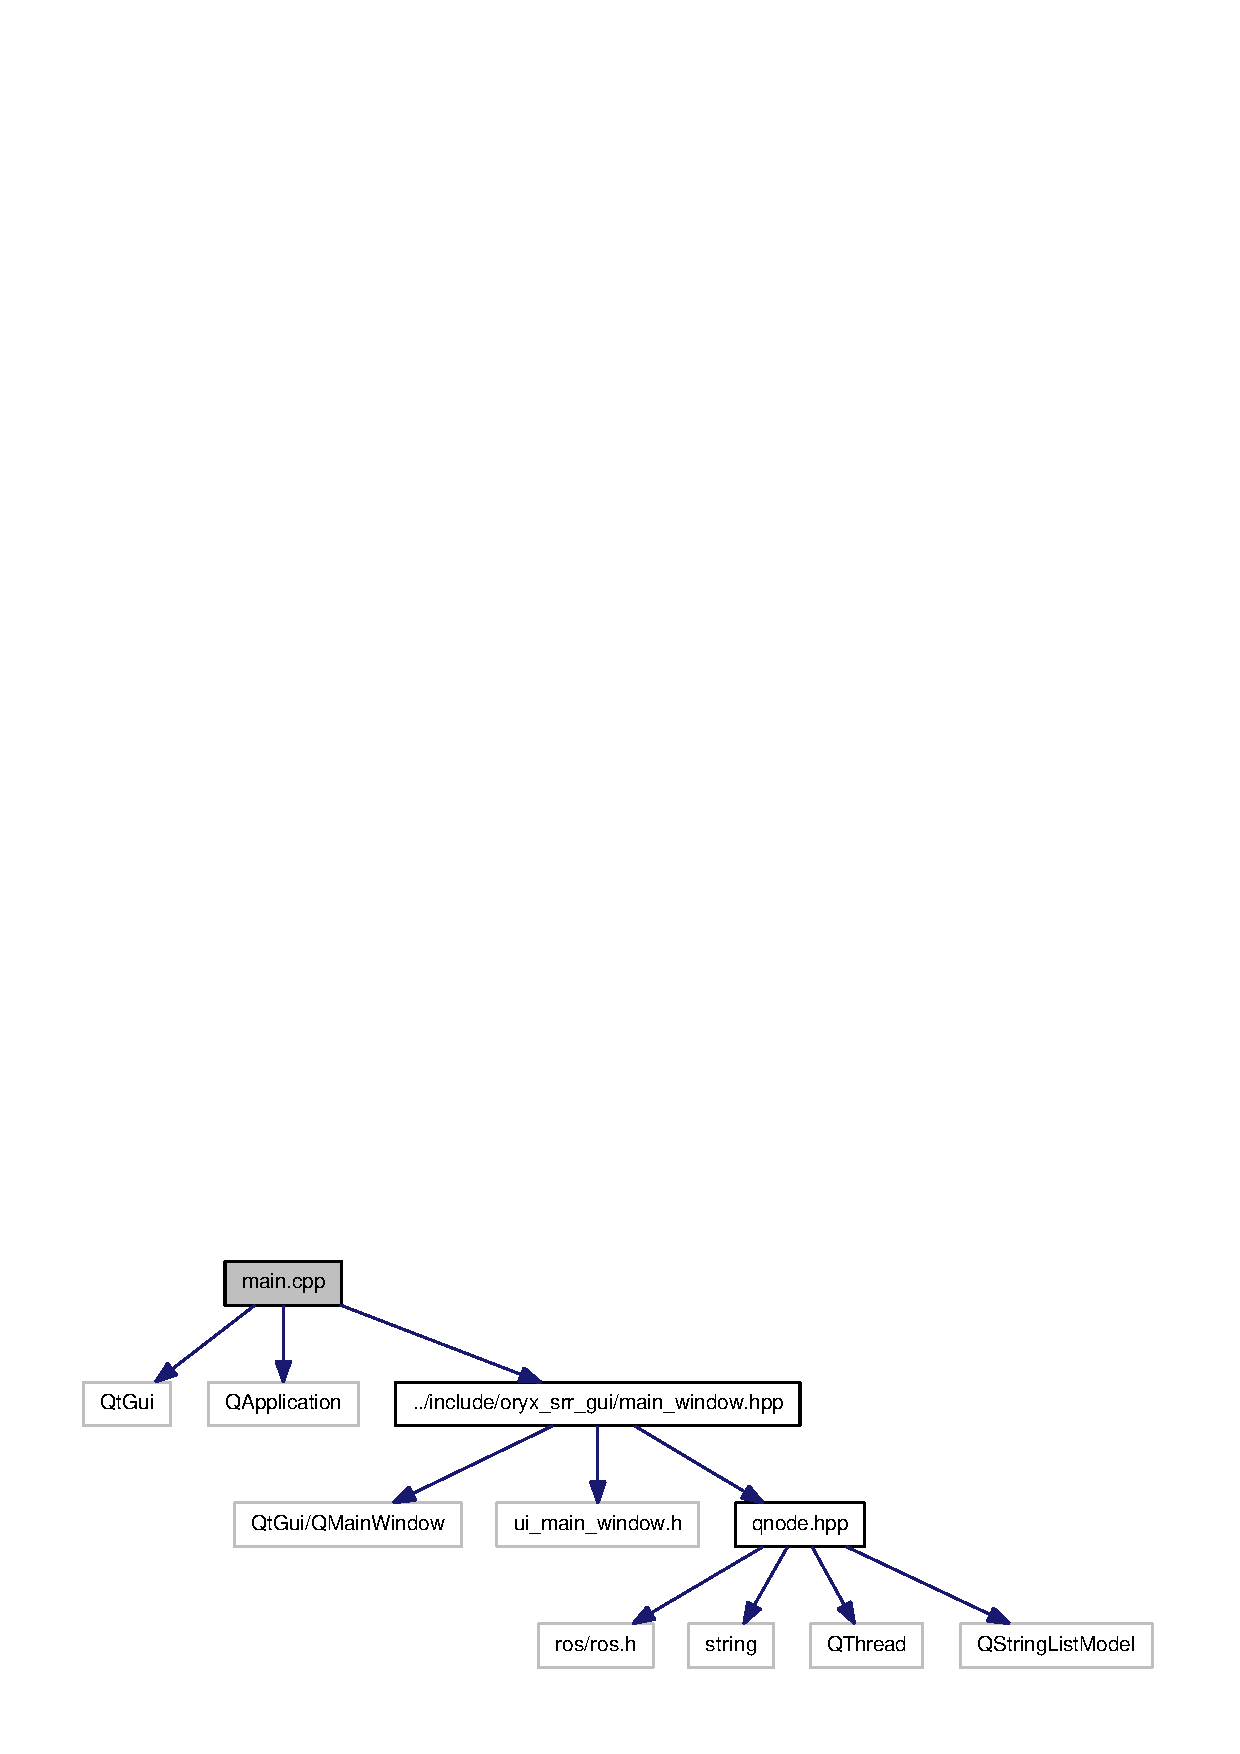
\includegraphics[width=350pt]{main_8cpp__incl}
\end{center}
\end{figure}
\subsection*{\-Functions}
\begin{DoxyCompactItemize}
\item 
int {\bf main} (int argc, char $\ast$$\ast$argv)
\end{DoxyCompactItemize}


\subsection{\-Detailed \-Description}
\-Qt based gui. \begin{DoxyDate}{\-Date}
\-November 2010 
\end{DoxyDate}


\-Definition in file {\bf main.\-cpp}.



\subsection{\-Function \-Documentation}
\index{main.\-cpp@{main.\-cpp}!main@{main}}
\index{main@{main}!main.cpp@{main.\-cpp}}
\subsubsection[{main}]{\setlength{\rightskip}{0pt plus 5cm}int {\bf main} (
\begin{DoxyParamCaption}
\item[{int}]{argc, }
\item[{char $\ast$$\ast$}]{argv}
\end{DoxyParamCaption}
)}\label{main_8cpp_a3c04138a5bfe5d72780bb7e82a18e627}


\-Definition at line 20 of file main.\-cpp.


\section{main\-\_\-window.\-cpp \-File \-Reference}
\label{main__window_8cpp}\index{main\-\_\-window.\-cpp@{main\-\_\-window.\-cpp}}


\-Implementation for the qt gui.  


{\ttfamily \#include $<$\-Qt\-Gui$>$}\*
{\ttfamily \#include $<$\-Q\-Message\-Box$>$}\*
{\ttfamily \#include $<$iostream$>$}\*
{\ttfamily \#include \char`\"{}../include/oryx\-\_\-srr\-\_\-gui/main\-\_\-window.\-hpp\char`\"{}}\*
\-Include dependency graph for main\-\_\-window.\-cpp\-:
\nopagebreak
\begin{figure}[H]
\begin{center}
\leavevmode
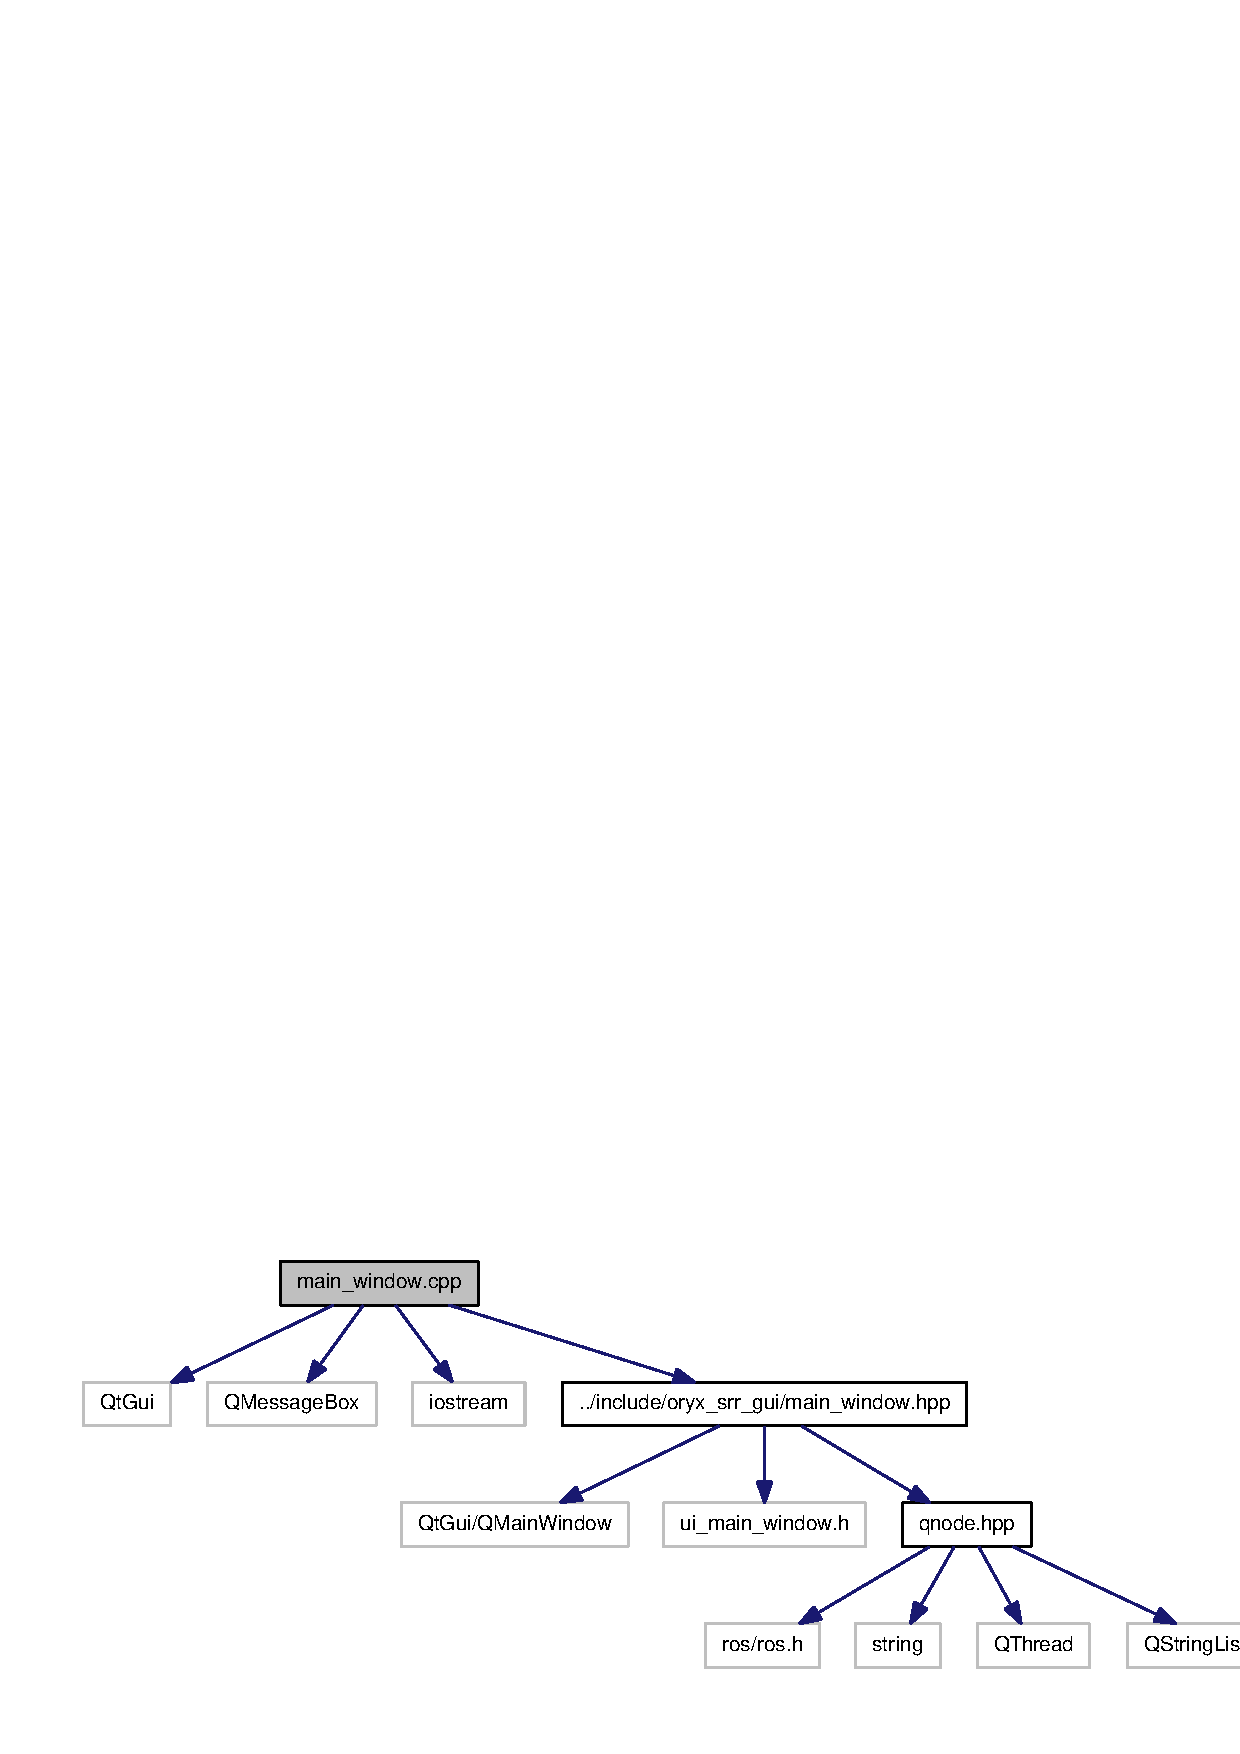
\includegraphics[width=350pt]{main__window_8cpp__incl}
\end{center}
\end{figure}
\subsection*{\-Namespaces}
\begin{DoxyCompactItemize}
\item 
namespace {\bf oryx\-\_\-srr\-\_\-gui}
\end{DoxyCompactItemize}


\subsection{\-Detailed \-Description}
\-Implementation for the qt gui. \begin{DoxyDate}{\-Date}
\-February 2011 
\end{DoxyDate}


\-Definition in file {\bf main\-\_\-window.\-cpp}.


\section{main\-\_\-window.\-hpp \-File \-Reference}
\label{main__window_8hpp}\index{main\-\_\-window.\-hpp@{main\-\_\-window.\-hpp}}


\-Qt based gui for \doxyref{oryx\-\_\-srr\-\_\-gui}{p.}{namespaceoryx__srr__gui}.  


{\ttfamily \#include $<$\-Qt\-Gui/\-Q\-Main\-Window$>$}\*
{\ttfamily \#include \char`\"{}ui\-\_\-main\-\_\-window.\-h\char`\"{}}\*
{\ttfamily \#include \char`\"{}qnode.\-hpp\char`\"{}}\*
\-Include dependency graph for main\-\_\-window.\-hpp\-:
\nopagebreak
\begin{figure}[H]
\begin{center}
\leavevmode
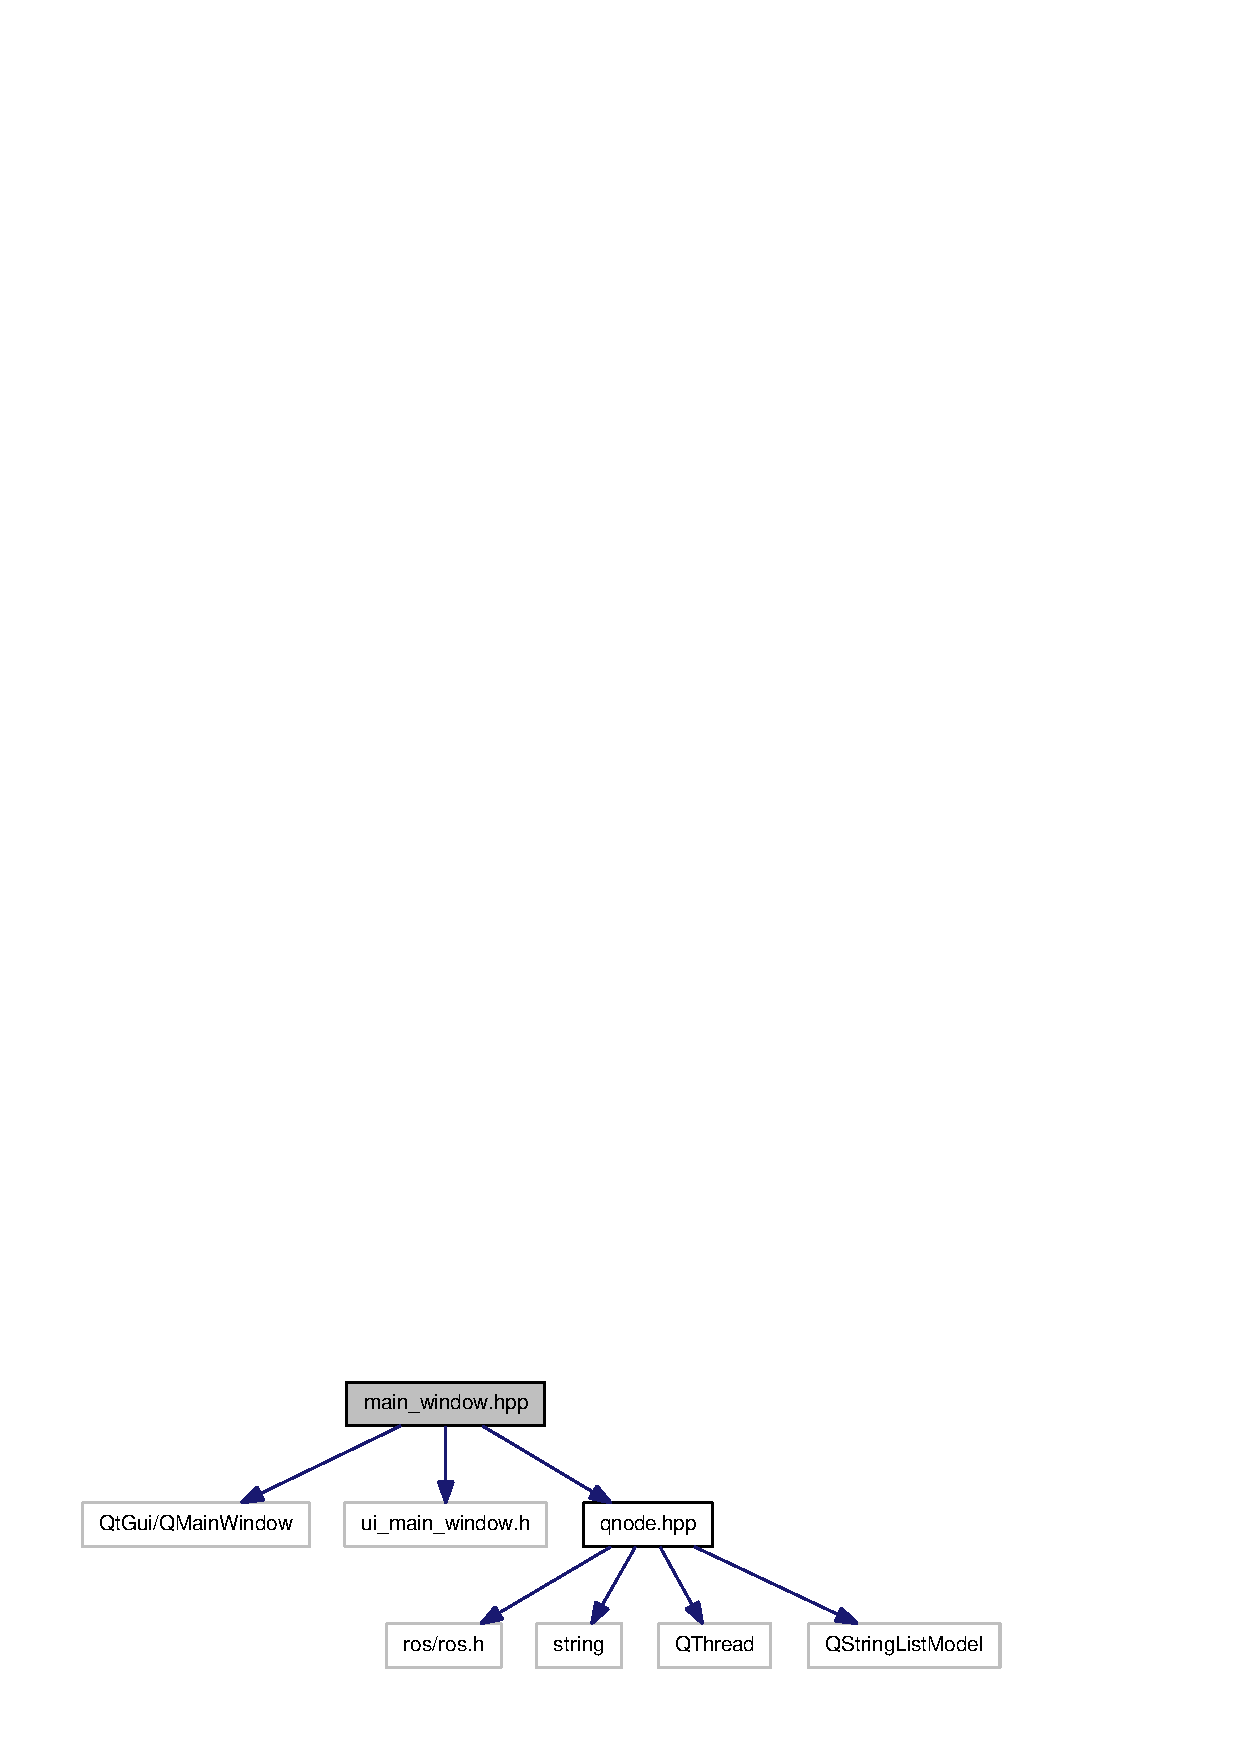
\includegraphics[width=350pt]{main__window_8hpp__incl}
\end{center}
\end{figure}
\-This graph shows which files directly or indirectly include this file\-:
\nopagebreak
\begin{figure}[H]
\begin{center}
\leavevmode
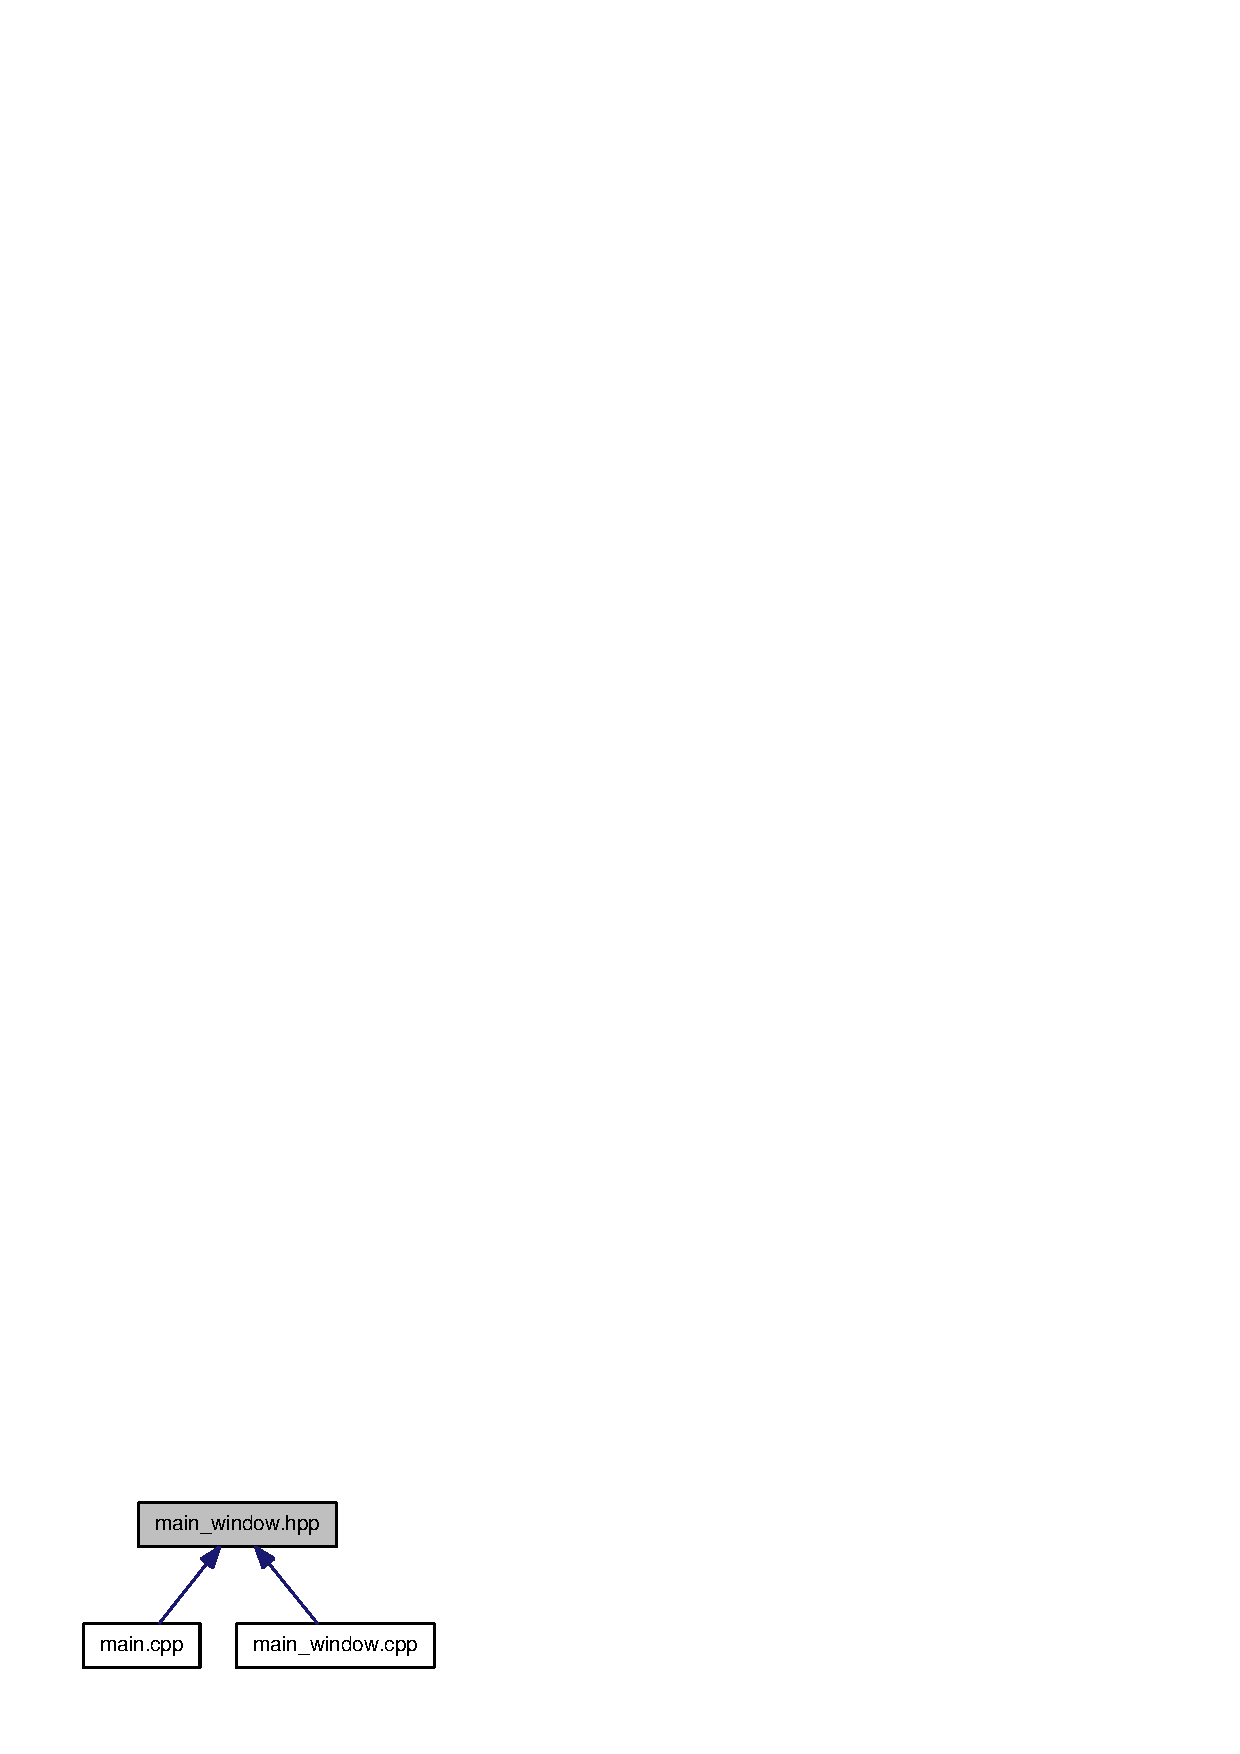
\includegraphics[width=212pt]{main__window_8hpp__dep__incl}
\end{center}
\end{figure}
\subsection*{\-Classes}
\begin{DoxyCompactItemize}
\item 
class {\bf oryx\-\_\-srr\-\_\-gui\-::\-Main\-Window}
\begin{DoxyCompactList}\small\item\em \-Qt central, all operations relating to the view part here. \end{DoxyCompactList}\end{DoxyCompactItemize}
\subsection*{\-Namespaces}
\begin{DoxyCompactItemize}
\item 
namespace {\bf oryx\-\_\-srr\-\_\-gui}
\end{DoxyCompactItemize}


\subsection{\-Detailed \-Description}
\-Qt based gui for \doxyref{oryx\-\_\-srr\-\_\-gui}{p.}{namespaceoryx__srr__gui}. \begin{DoxyDate}{\-Date}
\-November 2010 
\end{DoxyDate}


\-Definition in file {\bf main\-\_\-window.\-hpp}.


\section{mainpage.\-dox \-File \-Reference}
\label{mainpage_8dox}\index{mainpage.\-dox@{mainpage.\-dox}}

\section{qnode.\-cpp \-File \-Reference}
\label{qnode_8cpp}\index{qnode.\-cpp@{qnode.\-cpp}}


\-Ros communication central!  


{\ttfamily \#include $<$ros/ros.\-h$>$}\*
{\ttfamily \#include $<$ros/network.\-h$>$}\*
{\ttfamily \#include $<$string$>$}\*
{\ttfamily \#include $<$std\-\_\-msgs/\-String.\-h$>$}\*
{\ttfamily \#include $<$sstream$>$}\*
{\ttfamily \#include \char`\"{}../include/oryx\-\_\-srr\-\_\-gui/qnode.\-hpp\char`\"{}}\*
\-Include dependency graph for qnode.\-cpp\-:
\nopagebreak
\begin{figure}[H]
\begin{center}
\leavevmode
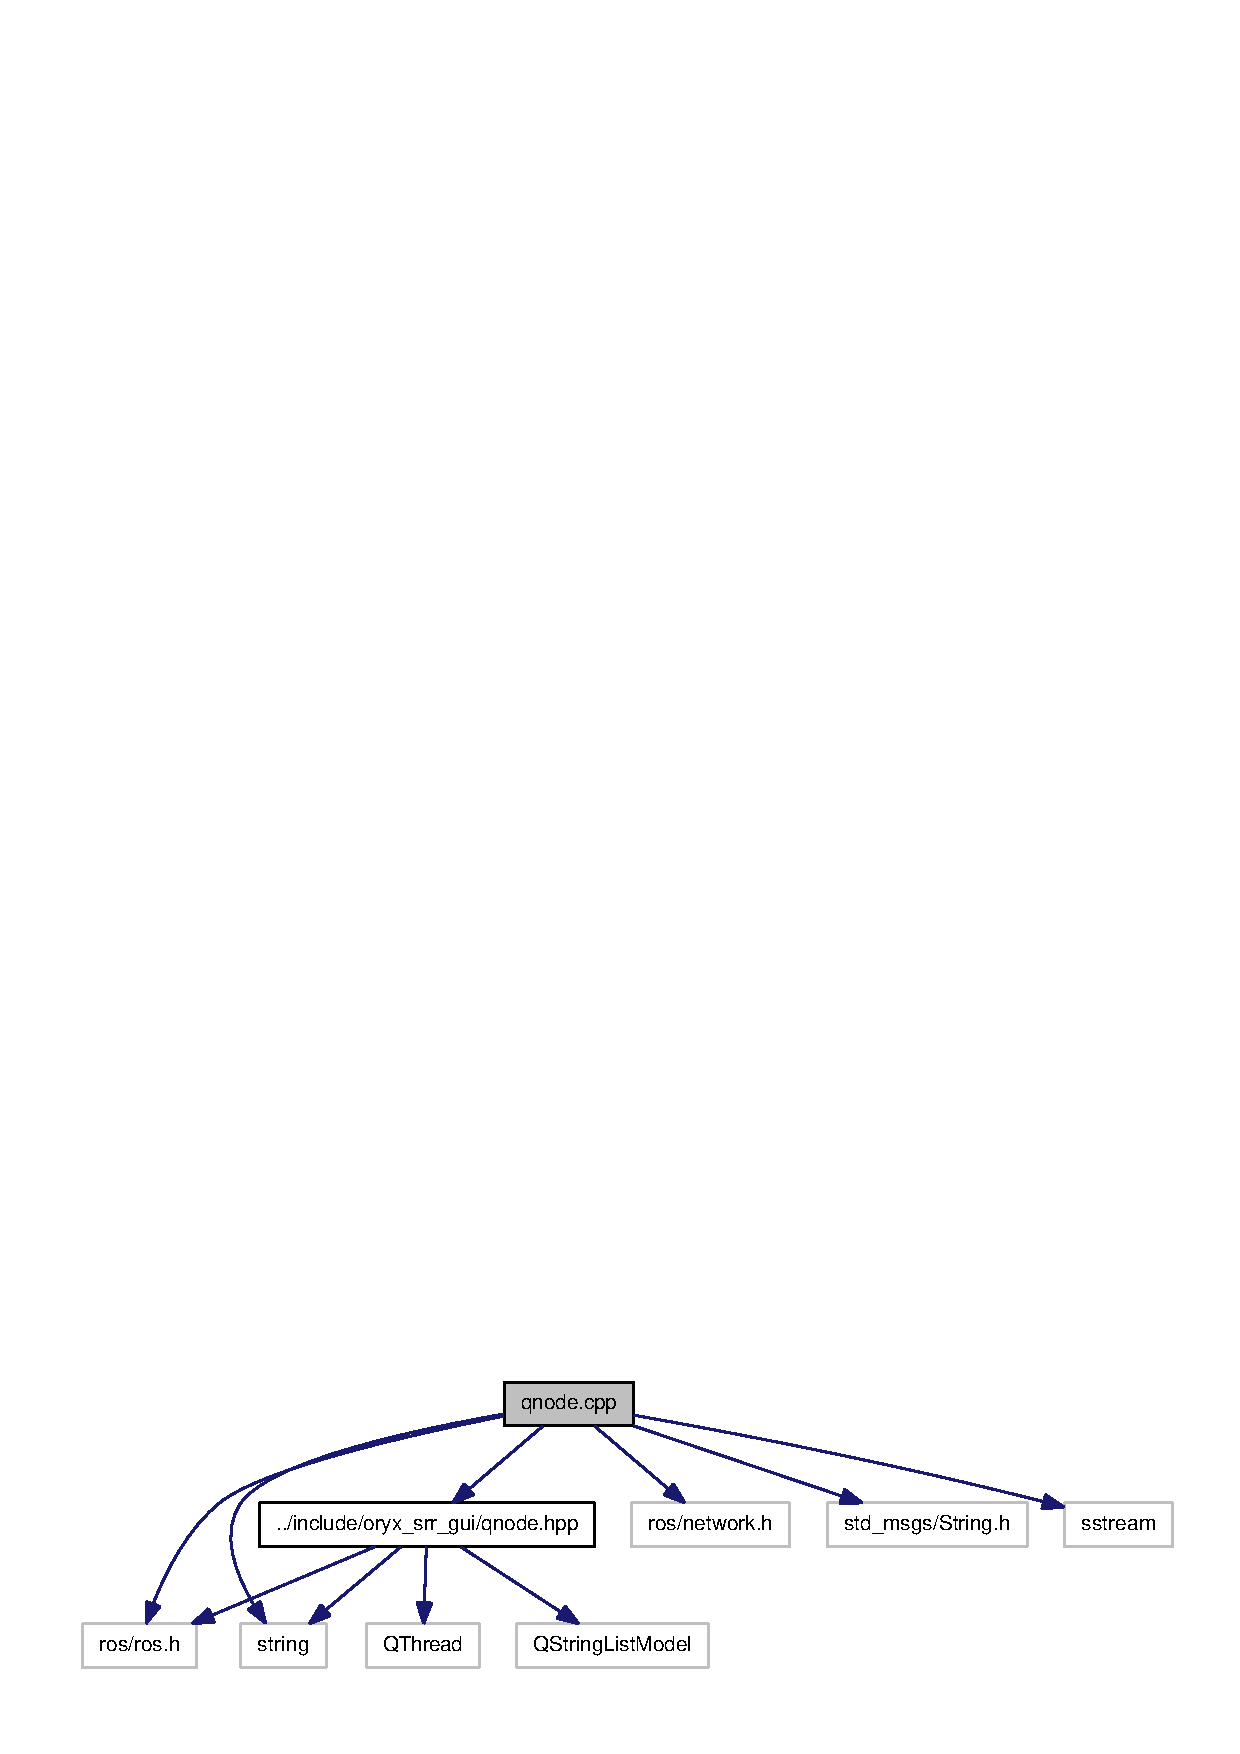
\includegraphics[width=350pt]{qnode_8cpp__incl}
\end{center}
\end{figure}
\subsection*{\-Namespaces}
\begin{DoxyCompactItemize}
\item 
namespace {\bf oryx\-\_\-srr\-\_\-gui}
\end{DoxyCompactItemize}


\subsection{\-Detailed \-Description}
\-Ros communication central! \begin{DoxyDate}{\-Date}
\-February 2011 
\end{DoxyDate}


\-Definition in file {\bf qnode.\-cpp}.


\section{qnode.\-hpp \-File \-Reference}
\label{qnode_8hpp}\index{qnode.\-hpp@{qnode.\-hpp}}


\-Communications central!  


{\ttfamily \#include $<$ros/ros.\-h$>$}\*
{\ttfamily \#include $<$string$>$}\*
{\ttfamily \#include $<$\-Q\-Thread$>$}\*
{\ttfamily \#include $<$\-Q\-String\-List\-Model$>$}\*
\-Include dependency graph for qnode.\-hpp\-:
\nopagebreak
\begin{figure}[H]
\begin{center}
\leavevmode
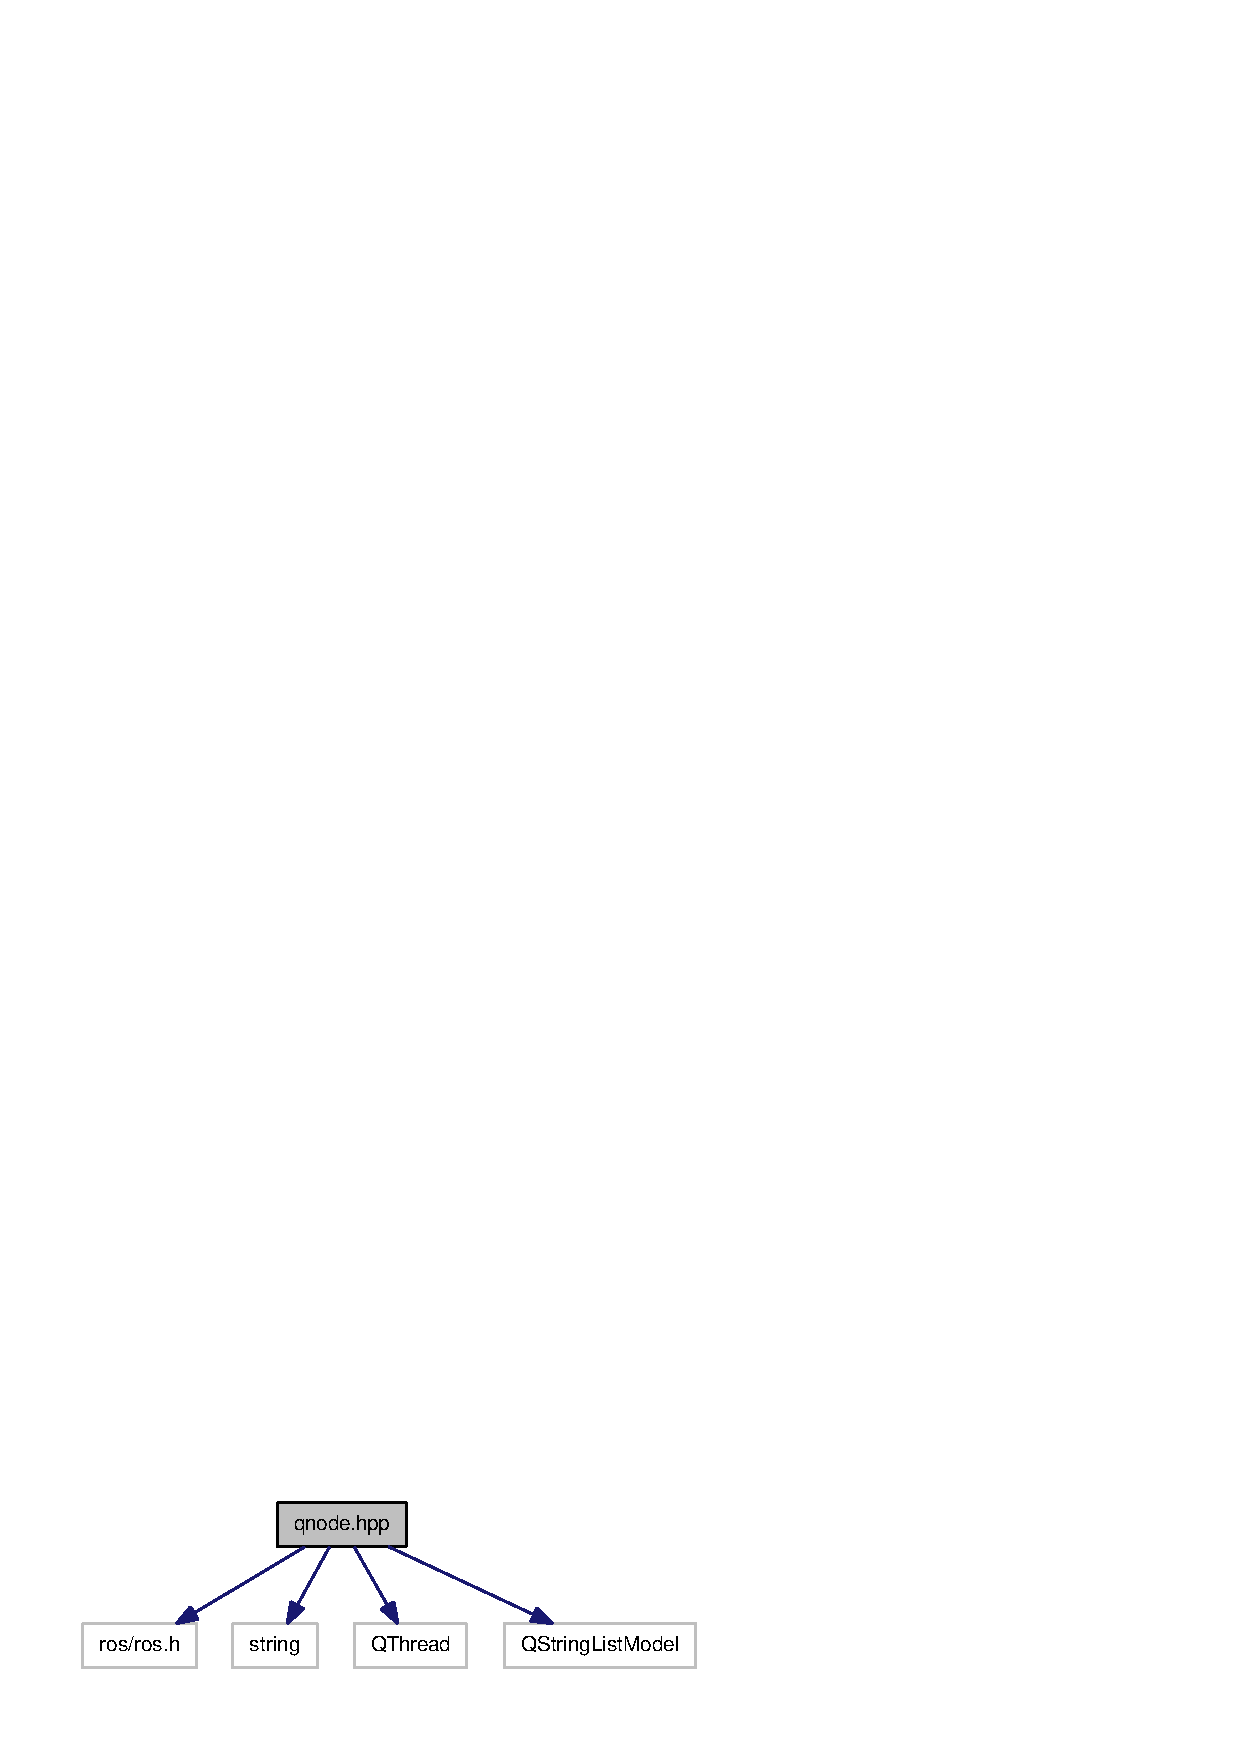
\includegraphics[width=338pt]{qnode_8hpp__incl}
\end{center}
\end{figure}
\-This graph shows which files directly or indirectly include this file\-:
\nopagebreak
\begin{figure}[H]
\begin{center}
\leavevmode
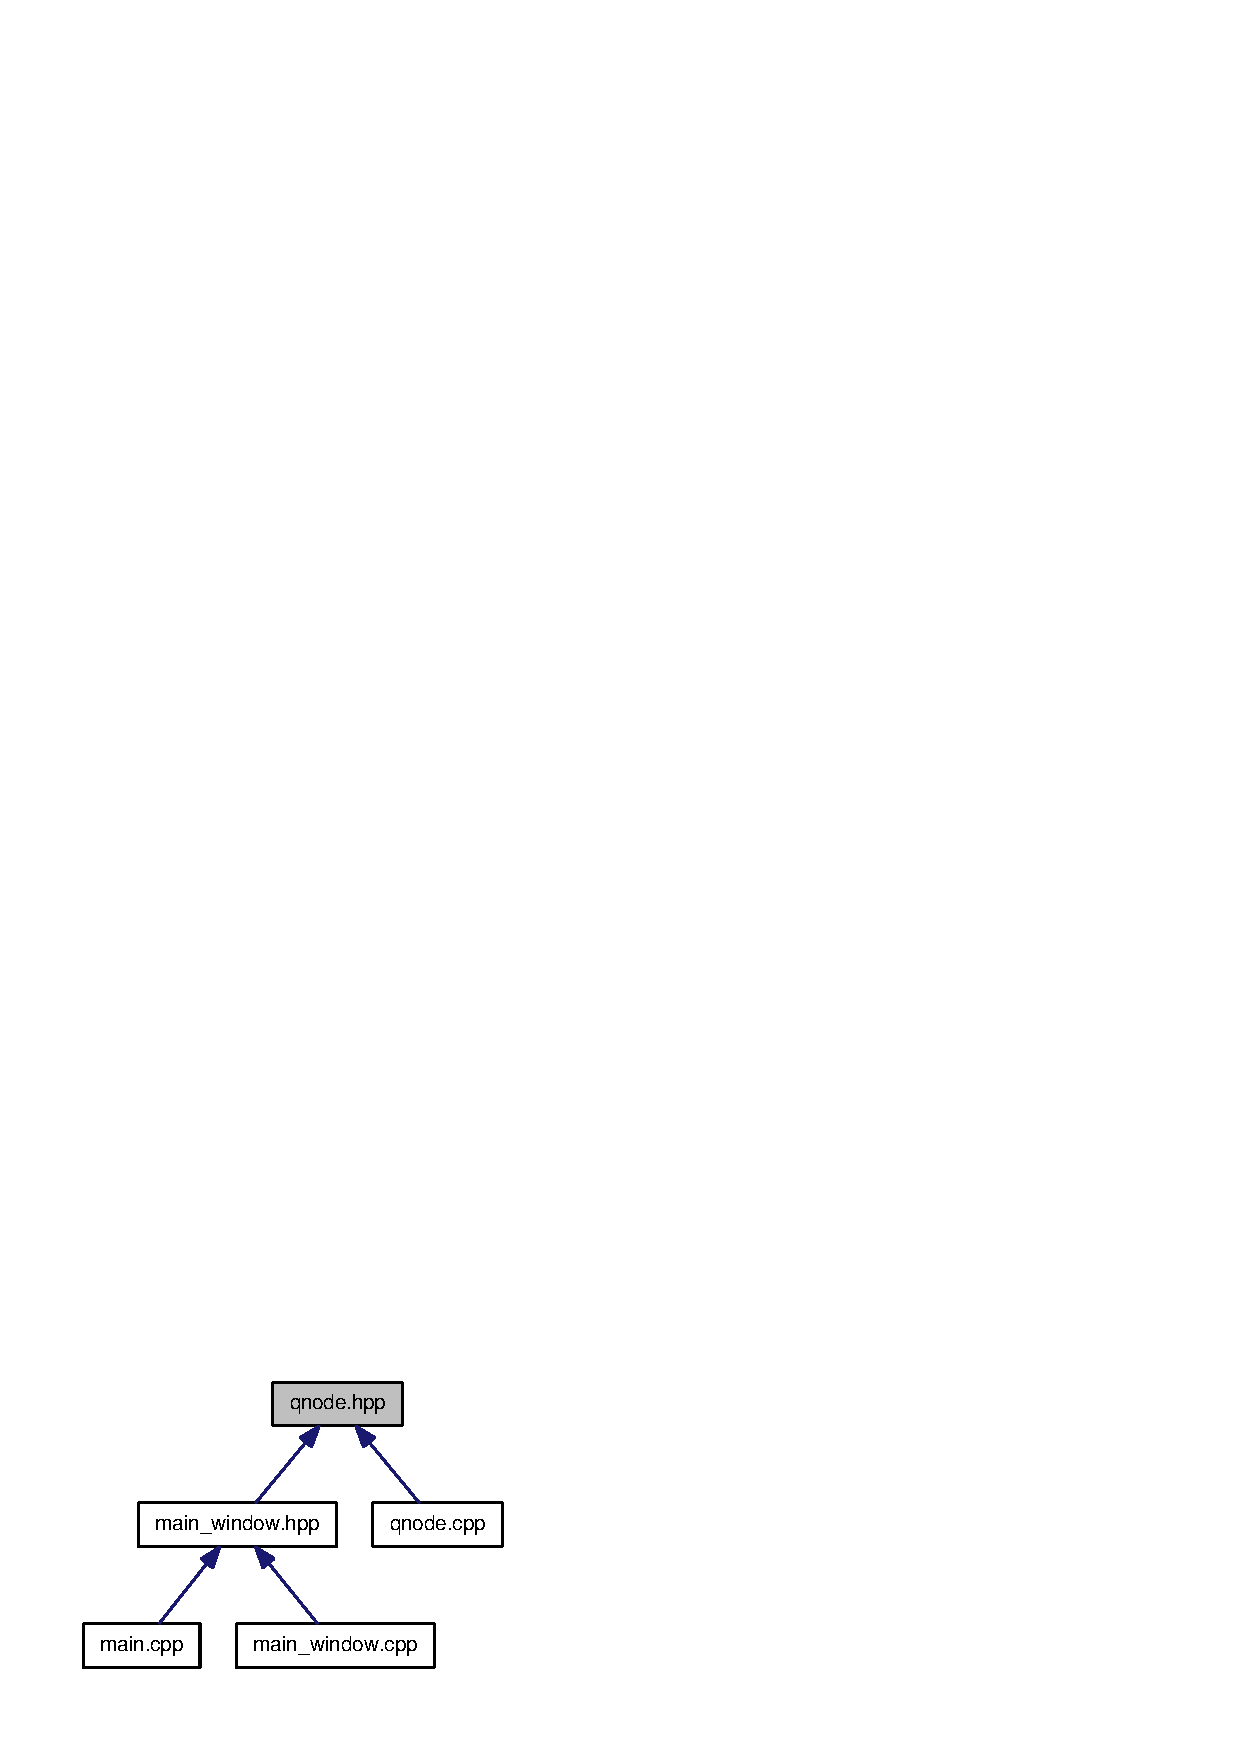
\includegraphics[width=245pt]{qnode_8hpp__dep__incl}
\end{center}
\end{figure}
\subsection*{\-Classes}
\begin{DoxyCompactItemize}
\item 
class {\bf oryx\-\_\-srr\-\_\-gui\-::\-Q\-Node}
\end{DoxyCompactItemize}
\subsection*{\-Namespaces}
\begin{DoxyCompactItemize}
\item 
namespace {\bf oryx\-\_\-srr\-\_\-gui}
\end{DoxyCompactItemize}


\subsection{\-Detailed \-Description}
\-Communications central! \begin{DoxyDate}{\-Date}
\-February 2011 
\end{DoxyDate}


\-Definition in file {\bf qnode.\-hpp}.


\printindex
\end{document}
